\chapter{Preliminaries}
\section{Preliminaries} % (fold)
\label{sec:preliminaries}
\subsection{Definitions, notations} % (fold)
\label{sub:definitions_notations}
A Finite Element in $\mathbb{R}^n$ is defined by the following triple $(K, P_K, \Sigma) $:

\vspace{5pt}
\noindent
$K$ is an open non empty domain of $\mathbb{R}^n$ with Lipschitz--continuous 
boundary.\\[5pt]
\noindent
$P_K$ is a finite--dimensional space of real--valued functions defined over $K$.\\[5pt]
\noindent
$\Sigma$ is a finite set of linearly independent linear functionals acting 
on a functional space containing $P_K$. The elements of $\Sigma$ are often
referred to as  \emph{degrees of freedom} or \emph{moments} of the Finite
Element.
% subsection definiciones_notaciones (end)

\subsection{Polynomials} % (fold)
\label{sub:polynomials}
The finite elements involved in this Thesis are built with piecewise
polynomial functions or rational functions (that is, quotients of polynomials).
For that reason we state some handy notations here.
\begin{defi}
\begin{IEEEeqnarray*}{rCl}
	P_k & = & \{\,\mbox{polynomials of degree less than or equal to k}\,\}\\[5pt]
	\tilde{P}_k & = & \{\,\mbox{homogeneous polynomials of degree k}\,\}
\end{IEEEeqnarray*}
In the case of a line segment \emph{e} or a subdomain \emph{f} of a plane (typically
an edge or a face of a polyhedron) we will write
\begin{IEEEeqnarray*}{rCl}
	P_k (e) & = & \{\,\mbox{polynomials of maximum degree k in arc length on e}\,\}\\[5pt]
	P_k (f) & = & \{\,\mbox{polynomials of maximum degree k in $\xi_1$,$\xi_2$ on f}\,\}
\end{IEEEeqnarray*}
where we have used an orthogonal coordinate system $(\xi_1,\xi_2)$ in the plane
containing $f$.\\[5pt]
Moreover, we will make the identifications
\begin{IEEEeqnarray*}{rClCrCl}
	P_k(e) & = & \{p|_e\,:\,p\in P_k\} &\quad\mbox{ and }\quad&P_k(f)
	& = & \{p|_f\,:\,p\in P_k\}.
\end{IEEEeqnarray*}
\end{defi}
% subsection polynomials (end)
\subsection{Functional Spaces. Trace Spaces.} % (fold)
\label{sub:functional_spaces_trace_spaces}
\begin{defi}
\begin{IEEEeqnarray*}{rCl}
	W^p(\emph{\textbf{curl}}, K) &=& \{ \emph{\textbf{u}}\in W^{1,p}(K)^3\,:\,\emph{
	\curl}\emph{\textbf{u}}\in W^{1,1}(K)^3\}\\
	\label{normaWpcurl}\yesnumber \|\emph{\textbf{u}}\|_{_{W^p(\emph{\textbf{curl}}, K)}} &=& 
	\|\emph{\textbf{u}}\|_{_{W^{1,p}(K)}} +
	\| \emph{\curl}\emph{\textbf{u}} \|_{_{W^{1,1}(K)}}. 
\end{IEEEeqnarray*}
\end{defi}
% subsection functional_spaces_trace_spaces (end)

\referencePrismTikz
\subsection{Definici\'on del \emph{edge element} en prismas} % (fold)
\label{sub:defEdgeElement}
Now we introduce two polynomial spaces which will be used to construct 
the edge elements on the reference prism (Figure~\ref{reference_prism}).
\begin{defi} $R_k(\hat{T})$ is the space of polynomials defined over the
triangle $\hat{T}$ given by
\begin{IEEEeqnarray}{rClCrCl}
	R_k(\hat{T}) & := & P_{k-1}(\hat{T})^2 \oplus S_k(\hat{T}) &\quad&  k&\geqslant&1
\end{IEEEeqnarray}
where
\begin{IEEEeqnarray}{rClCrCl}
	\label{defSk}
	S_k(\hat{T}) 		& := & \{ \emph{\textbf{p}}\in \tilde{P}_k^2 \,:\;\emph{\textbf{p}}\cdot\emph{\textbf{x}} = 0\}$\quad$\emph{\textbf{x}}	& = & (x_1, x_2).
\end{IEEEeqnarray}
\end{defi}
\noindent In order to establish unisolvence we need to calculate
$\dim\left(R_k(\hat{T}) \otimes P_k(\hat{I})\right)$.
\begin{IEEEeqnarray*}{rCl}
	\dim\left(R_k(\hat{T}) \otimes P_k(\hat{I})\right) 
	& = & \dim\left(R_k(\hat{T})\right)	\dim\left(P_k(\hat{I})\right) \\
	& = & \dim\left(R_k(\hat{T})\right)	(k+1).
\end{IEEEeqnarray*}
\begin{IEEEeqnarray*}{rCl}
	\dim\left(R_k(\hat{T})\right) 
	& = & \dim\left(P_{k-1}(\hat{T})^2 \oplus S_k(\hat{T}) \right)\\
	& = & 2\dim\left(P_{k-1}(\hat{T})\right) + \dim\left(S_k(\hat{T}) \right)\\
	& = & k(k+1) + \dim\left(S_k(\hat{T}) \right).
\end{IEEEeqnarray*}
Para la dimensi\'on de $S_k(\hat{T})$:
\begin{IEEEeqnarray*}{rCl}
S_k(\hat{T}) = \{ \textbf{p} \in \widetilde{P}_k^2 \, : \, \textbf{p}\cdot\textbf{x} = 0 \}.
\end{IEEEeqnarray*}
Consid\'erese
\begin{IEEEeqnarray*}{lll}
	\phi\,:\,\widetilde{P}_k^2 & \longrightarrow & \widetilde{P}_{k+1}\\
	\phi(\textbf{p}) 	& := & \textbf{p}\cdot\textbf{x}\\
						& := & x_1p_1 + x_2p_2.
\end{IEEEeqnarray*}
Resulta
\begin{IEEEeqnarray*}{rCl}
	S_k(\hat{T}) 		& = & \ker(\phi)\\
	\dim(S_k(\hat{T})) 	& = & \dim(\widetilde{P}_k^2) - \dim(\img(\phi)).
\end{IEEEeqnarray*}
cualquier $p \in \widetilde{P}_{k+1}$ es
\begin{IEEEeqnarray*}{rCl}
	x_1(a_{k+1,0} x_1^k + a_{k,1} x_1^{k-1}x_2 + \ldots + a_{1,k} x_2^k) + x_2(a_{0,k+1} x_2^k)
		& = & x_1p_1 + x_2p_2
\end{IEEEeqnarray*}
en donde precisamente $p_1$ y $p_2$ pertenecen a $\widetilde{P}_k$, es decir que $\phi$ es
sobreyectiva. Volviendo:
\begin{IEEEeqnarray*}{rCl}
	\dim(S_k(\hat{T})) 	& = & \dim(\widetilde{P}_k^2) - \dim(\widetilde{P}_{k+1})\\
					 		& = & 2 \dim(\widetilde{P}_k) - \dim(\widetilde{P}_{k+1})\\
					 		& = & 2 (k+1) - (k+2)\\
					 		& = & k,
\end{IEEEeqnarray*}
entonces
\begin{IEEEeqnarray*}{rCl}
	\dim\left(R_k(\hat{T})\right) 	& = & k(k+1) + k\\
					 					& = & k(k+2)
\end{IEEEeqnarray*}
y finalmente
\begin{IEEEeqnarray*}{rCl}
	\dim\left(R_k(\hat{T}) \otimes P_k(\hat{I})\right) 
		& = & k(k+1)(k+2).
\end{IEEEeqnarray*}
($\dim\left(P_K\right) = 3\frac{k(k+1)(k+2)}{2}$).
\begin{defi}
\label{edgeelement} Dado un natural $k$, los \emph{edge elements}
de grado $k$ en el prisma de referencia se definen por lo
si\-guien\-te:
\begin{enumerate}
	\item $\hat{K}$ es el prisma $\hat{T} \times \hat{I}$ donde $\hat{T} = 
	\{ 0 < x + y < 1 \}$ e $\hat{I} = \{ 0<z<1 \} $.
	\item El espacio de polinomios  $P_{\hat{K}}$ es
		\begin{IEEEeqnarray*}{rCl}
		 	P_{\hat{K}} & = & R_k(\hat{T}) \otimes P_k(\hat{I}) \times 
			P_k(\hat{T}) \otimes P_{k-1}(\hat{I}).
		 \end{IEEEeqnarray*} 
	\item Los grados de libertad son:
\begin{IEEEeqnarray}{ll}
	\label{momentos1hcurl} \int\limits_{a} \textbf{u} \cdot \boldsymbol{\tau} \,q\, ds  
		& q\in P_{k-1}\textrm{,} \\
	\IEEEeqnarraymulticol{2}{l}{\nonumber\textrm{ para cada arista $a$ con tangente unitaria } \boldsymbol{\tau} \textrm{;}}\\[8pt]
	\label{momentos2hcurl} \int\limits_{f} \textbf{u} \times \boldsymbol{\nu} \cdot \boldsymbol{q}\,
	d\gamma\textrm{, } &\boldsymbol{q} = (q_1,q_2,0) \in P_{k-2}^2 \times \{ 0 \},\\ 
	\IEEEeqnarraymulticol{2}{l}{\nonumber\textrm{ para cada cara horizontal f con normal } \boldsymbol{\nu} = (0,0,\pm1) \textrm{;}}\\[8pt]
 	\label{momentos3hcurl} \int\limits_{f} \textbf{u} \times \boldsymbol{\nu} \cdot \boldsymbol{q}\,
 	d\gamma\textrm{, } &\boldsymbol{q} = (0,q_3,q_2) \in \{ 0 \} \times Q_{k-2,k-1} \times 
 	Q_{k-1,k-2}\textrm{, } \\
 	\IEEEeqnarraymulticol{2}{l}{\nonumber\textrm{ para la cara } f \subseteq \{ x=0 \} \textrm{ con normal }\boldsymbol{\nu} = (-1,0,0) \textrm{;}}\\[8pt]
 	\label{momentos4hcurl} \int\limits_{f} \textbf{u} \times \boldsymbol{n} \cdot \boldsymbol{q}\,
 	d\gamma\textrm{, } & \boldsymbol{q} = (q_3,0,q_1) \in Q_{k-2,k-1} \times \{ 0 \} \times
 	Q_{k-1,k-2},\\
 	\IEEEeqnarraymulticol{2}{l}{\nonumber\textrm{ para la cara }f \subseteq \{ y=0 \} \textrm{ con normal }\boldsymbol{n} = (0,-1,0) \textrm{;}}\\[8pt]
	\label{momentos5hcurl} \int\limits_{f} \textbf{u} \times \boldsymbol{n} \cdot \boldsymbol{q}\,
	d\gamma\textrm{, } & \boldsymbol{q} = (0,q_3,q_1) \in \{ 0 \} \times Q_{k-2,k-1} \times
	Q_{k-1,k-2}\textrm{, }\\
	\IEEEeqnarraymulticol{2}{l}{\nonumber\textrm{ para la cara }f \subseteq \{x+y=1\} \textrm{ con normal }\boldsymbol{n} = (1,1,0) \textrm{;}}\\[8pt]
 	\label{momentos6hcurl} \int\limits_{K} \textbf{u} \cdot \boldsymbol{q} \, d\textbf{x}\textrm{, }&\\
 	\IEEEeqnarraymulticol{2}{l}{\nonumber q_1, q_2 \in P_{k-2}(x,y) \otimes 
 		P_{k-2}(z)\textrm{, }q_3 \in P_{k-3}(x,y) \otimes P_{k-1}(z).}
\end{IEEEeqnarray}
\end{enumerate}
\end{defi}
\begin{ejemplo}[edge elements of degree 1]
\begin{IEEEeqnarray*}{rCl}
\hat{\textbf{u}}\,(\hat{x},\hat{y},\hat{z}) &=& 
\left(
	\begin{array}{c}
		a_1 + a_3\hat{y} + a_4\hat{z} + a_6\hat{y}\hat{z} \\[8pt]
		a_2 - a_3\hat{x} + a_5\hat{z} - a_6\hat{x}\hat{z} \\[8pt]
		a_7 + a_8\hat{x} + a_9\hat{y}
	\end{array}
\right)\\[8pt]
(\hat{\textbf{u}}\cdot\boldsymbol{\tau})|_{\boldsymbol{e}}
	&\in&\mathbb{P}_0
\end{IEEEeqnarray*}

\end{ejemplo}

Por la presencia de los momentos~(\ref{momentos1hcurl}) no se puede definir el interpolador para un campo arbitrario
en $H(\textbf{curl}, K)$, así que por eso to\-ma\-mos co\-mo hi\-pó\-te\-sis que sea $p>2$ (ver~\cite{monk}, página 134,
~\cite{adams}, Theorem 5.4).\\\\
En~\cite{nedelec2} se prueba que este elemento es $H(\textbf{curl})$--conforme y unisolvente. {\color{BrickRed}>Está
bien usar esta conformidad, siendo que restringimos a Wp?}\\[5pt]
El siguiente lemma será usado para demostrar el teorema de estabilidad en el elemento de referencia con un argumento de densidad. Para su demostración referimos a~\cite{adams}.
\begin{lemma}\label{lemaDensidad}
$C^\infty(\bar{K})^3$ es un subespacio denso de $\wpcurl{K}$ con la norma~(\ref{normaWpcurl}).
\end{lemma}
% subsection defEdgeElement (end)

\begin{lemma} From the Hdiv space on prisms ---> $\dim(P_{\hat{K}}) = k^2\,(k+2) + \frac{k\,(k+1)^2}{2}$
\end{lemma}
\begin{proof}
	From the definition of the discrete space, and the notation involved, it follows that for each
	$\textbf{p} = (p_1, p_2, p_3) \in  P_{\hat{K}}$ there are unique $q_1, q_2 \in 
	\mathcal{P}_{k-1}(x,y)\otimes\mathcal{P}_{k-1}(z)$, $q_3 \in \mathcal{P}_{k-1}(x,y)\otimes\mathcal{P}_{k}(z)$, and
	$h \in \tilde{\mathcal{P}}_{k-1}(x,y)\otimes\mathcal{P}_{k-1}(z)$ such that
	\begin{IEEEeqnarray*}{rCl}
									p_1(x, y, z) & = & q_1(x, y, z) + x\,h(x, y, z)\\
		\label{exprPrt} \yesnumber 	p_2(x, y, z) & = & q_2(x, y, z) + y\,h(x, y, z)\\
									p_3(x, y, z) & = & q_3(x, y, z)
	\end{IEEEeqnarray*} 
	so the number of coefficients defining \textbf{p} is
	\begin{IEEEeqnarray*}{rCl}
		2\,\frac{k\,(k+1)}{2}\,k + k^2 + \frac{k\,(k+1)}{2}\,(k+1) & &.
	\end{IEEEeqnarray*}
\end{proof}
\noindent Now a key result that establishes a relation between the interpolation operators. It will used as an important step in the proof of the stability of the
edge element on a prism.
\begin{lemma}\label{lema_pi_star_rot_u} Si $\pi$ es el operador de interpolaci\'on determinado por el elemento en
la Definici\'on~(\ref{edgeelement}) y $\pi^*$ es el operador de interpolaci\'on determinado por el elemento en la
Definici\'on~(\ref{defi_h_div_conforme}), entonces, para toda $\emph{\textbf{u}}$ tal que 
"existan las dos composiciones"
\begin{IEEEeqnarray}{rCl}
	\emph{\textbf{curl}}\,\pi \emph{\textbf{u}} &=& \pi^*\emph{\textbf{curl}}\,\emph{\textbf{u}}.
\end{IEEEeqnarray}
\end{lemma}
\begin{proof}
Vamos a usar la siguiente versión superficial del Teorema de Stokes. Sea dado un dominio Lipschitz acotado 
$S\subseteq\mathbb{R}^2$ con tangente unitaria $\boldsymbol{\tau}$ al borde $\partial S$. Para 
$\textbf{u} \in \mathcal{C}^1(\bar{S})^2 $ y $\phi \in \mathcal{C}^1(\bar{S})$ tenemos
\begin{IEEEeqnarray}{rCl}
	\int\limits_S \textbf{u} d\gamma & = &   %% HACER SEGUIR ACA
\end{IEEEeqnarray}
\end{proof}
\noindent The last result can be expressed saying that the following diagram commutes:
\begin{center}
		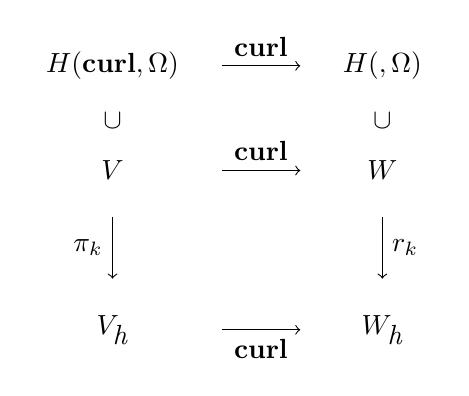
\begin{tikzpicture}[point/.style={circle, inner sep=0pt, minimum size=2pt,fill=red}]
			\matrix[column sep = 1.82mm, row sep = 1.1mm, ampersand replacement = \&] {
			 \node {$\text{H}(\textbf{curl},\Omega)$}; 	
			  \& \node (n0) {};
			  \& \node 		{};
			  \& \node (n1) {};
			  \& \node (n2) {};
			  \& \node {$\text{H}(\Div, \Omega)$}; \\
			 \node (n3)	{}; \&\&\&\&\& \node (n5) 	{}; \\
			 \node (n4)	{}; \&\&\&\&\& \node (n6) 	{}; \\  
			 \node (v)	{$V$}; \&\node(fromV){};\&\&\&\node(toW){};\& \node (w) {$W$}; \\
			 \node (n7)	{}; \&\&\&\&\& \node (n8)	{}; \\ 
			 \node 		{}; \&\&\&\&\& \node 	 	{}; \\ 
			 \node 		{}; \&\&\&\&\& \node 	 	{}; \\ 
			 \node (n11)	{}; \&\&\&\&\& \node (n12) {}; \\ 
			 \node {$V_{\textit{h}} $}; 								
			  \& \node (n13) {};
			  \& \node 		 {};
			  \& \node (n14) {};
			  \& \node (n15) {};
			  \& \node (n16) {}; 
			 \node {$W_{\textit{h}} $}; \\
			 };
			\draw[->] (n0) to node[above] {$\textbf{curl}$} (n2); 
			\draw[->] (fromV) to node[above] {$\textbf{curl}$} (toW); 
			\draw[white] (n3) to node {{\color{black}$\cup$}} (n4);
			\draw[white] (n5) to node {{\color{black}$\cup$}} (n6);
			\draw[->] (n7) to node[left] {$\pi_k$} (n11); 
			\draw[->] (n8) to node[right] {$\boldsymbol{r}_k$} (n12); 
			\draw[->] (n13) to node[below] {$\textbf{curl}$} (n15); 
		\end{tikzpicture}
	\end{center}

% subsection definition_of_the_h_div_element (end)

\subsection{Transformaciones entre prismas} % (fold)
\label{sub:transformaciones_entre_prismas}
Consideremos la aplicación $\hat{\textbf{x}}\longmapsto{\textbf{x}} = 
F_K(\hat{\textbf{x}})$, en donde $F_K = M\hat{\textbf{x}} + \textbf{x}_0$, que transforma
$\hat{K}$ en un elemento $K$ de la malla y $M$ es inversible y tiene determinante 
de signo constante.
Si tenemos una función escalar $\hat{p} \in H^1(\hat{K})$ definimos $p$ en $K$ por
\begin{IEEEeqnarray}{rCl}
	\label{transfEscalar} p\circ F_K & = & \hat{p}.
\end{IEEEeqnarray}
Then, with multiindex notation, for $F_K = \diag{h_1}{h_2}{h_3}$:
\begin{IEEEeqnarray*}{rCl}
	\partial^\alpha \hat{u} (\hat{\textbf{x}})&=&
		h^\alpha\partial^\alpha u(F_K(\hat{\textbf{x}})).
\end{IEEEeqnarray*}
Como $\nabla p = M^{-t}\hat{\nabla} \hat{p} \circ F_K^{-1}$, entonces resulta 
$p \in H^1(K)$.
Ahora tomemos $\hat{\textbf{u}} \in H(curl, \hat{K})$. Buscamos asociarle una
$\textbf{u}$ en $K$. Como para $\hat{p}$ y $p$ como recién vale
$\nabla p \in H(curl, K)$ y $\hat{\nabla} \hat{p} \in H(curl, \hat{K})$, la igualdad
anterior nos sugiere la transformación de $\hat{\textbf{u}}$ a $\textbf{u}$. En efecto
\begin{IEEEeqnarray}{rCl}
	\label{transfHcurl} \textbf{u}\circ F_K & = & M^{-t}\hat{\textbf{u}}.
\end{IEEEeqnarray} 
Con esta definición tenemos $\textbf{u}\in H(\textbf{curl}, K)$ y además
\begin{IEEEeqnarray}{rCl}
	\label{transfCurl} (\textbf{curl}\,\textbf{u})\circ F_K & = & 
	\frac{1}{\det M} M (\hat{\textbf{curl}}\,\hat{\textbf{u}}).
\end{IEEEeqnarray}
Transformación en $H(\dvg)$. Since $F_K$ is affine
\begin{IEEEeqnarray}{rCl}
	\label{transfDiv} \textbf{u}\circ F_K & = & 
	\frac{1}{\det M} M \hat{\textbf{u}}.
\end{IEEEeqnarray}
With~(\ref{transfDiv})
\begin{IEEEeqnarray*}{rCl}
	\|\hat{\textbf{v}}\|^2_{L^2(\hat{K})}
	&=&	\sum_{1\leqslant i\leqslant 3}\|\hat{v}_i\|^2_{0,\hat{K}}\\[7pt]
	&=& \sum_{1\leqslant i\leqslant 3}\frac{h_jh_k}{h_i}\,\|v_i\|^2_{0,K};\\[7pt]
	\|\hat{v}_i\|^2_{0,\hat{K}}&=&\frac{h_jh_k}{h_i}\,\|v_i\|^2_{0,K}
\end{IEEEeqnarray*}
where $\{i,j,k\} = \{1,2,3\}$.
\begin{lemma} For all $\tilde{\boldsymbol{\sigma}} \in H(\dvg, \tilde{K})$, $\boldsymbol{\sigma}$ results in
$H(\dvg, K)$ and in fact
\[
	\emph{div}\,\boldsymbol{\sigma}(\emph{\textbf{x}}) =
		\frac{1}{\det DF}\,\tilde{\emph{div}}\,\tilde{\boldsymbol{\sigma}}(\tilde{\emph{\textbf{x}}}).
\]
\end{lemma}
\begin{proof}
Observe that
\begin{IEEEeqnarray*}{rCl}
	trace(A\cdot B\cdot A^{-1}) &=& trace(B)\\
	\label{Piola}\yesnumber\boldsymbol{\sigma} \circ F & = & \frac{1}{\det(A)} A\,\tilde{\boldsymbol{\sigma}}\\
	\label{derivadaPiola}\yesnumber\tilde{D}\tilde{\boldsymbol{\sigma}}(\tilde{\textbf{x}}) & = &
		\det(A)\,A^{-1}\,D\boldsymbol{\sigma} (F(\tilde{\textbf{x}})) \,A.
\end{IEEEeqnarray*}
Then
\begin{IEEEeqnarray*}{rCl}
	\text{div}\,\boldsymbol{\sigma}(\textbf{x}) & = & trace(D\boldsymbol{\sigma} (\textbf{x}))\\
										& =	& \frac{1}{\det(A)}\,trace(A\,\tilde{D}\tilde{\boldsymbol{\sigma}} (F^{-1}(\textbf{x}))\,A^{-1})\\
										& =	& \frac{1}{\det(A)}\,\tilde{\text{div}}\,\tilde{\boldsymbol{\sigma}}(\tilde{\textbf{x}}).	
\end{IEEEeqnarray*}
\end{proof}

Todas estas igualdades se prueban en~\cite{monk}.\\\\
Citar de~\cite{monk}. 
\begin{lemma} The edge element interpolators satisfy
\begin{IEEEeqnarray}{rCl}\label{piTransformado}
	\hat{\pi}_k(\hat{\textbf{u}})(\hat{\textbf{x}}) & = & M^{t} \pi_k(\textbf{u})(\textbf{x}).
\end{IEEEeqnarray}
{\color{BrickRed} > lo probamos?}
\end{lemma}

% subsection transformaciones_entre_prismas (end)
% section preliminares (end)
	
